\section{Algorithms}\label{sec:algorithms}
This chapter describes how scalafmt formats Scala code.
We will see that scalafmt's design is inspired by ClangFormat and dartfmt.
However, we believe our design makes a valuable contribution in that it leverages functional programming principles to maximise code reuse and extensibility.

\subsection{Design}
Figure~\ref{fig:architecture} shows a broad architectural overview of scalafmt.
\begin{figure}
  \centering
  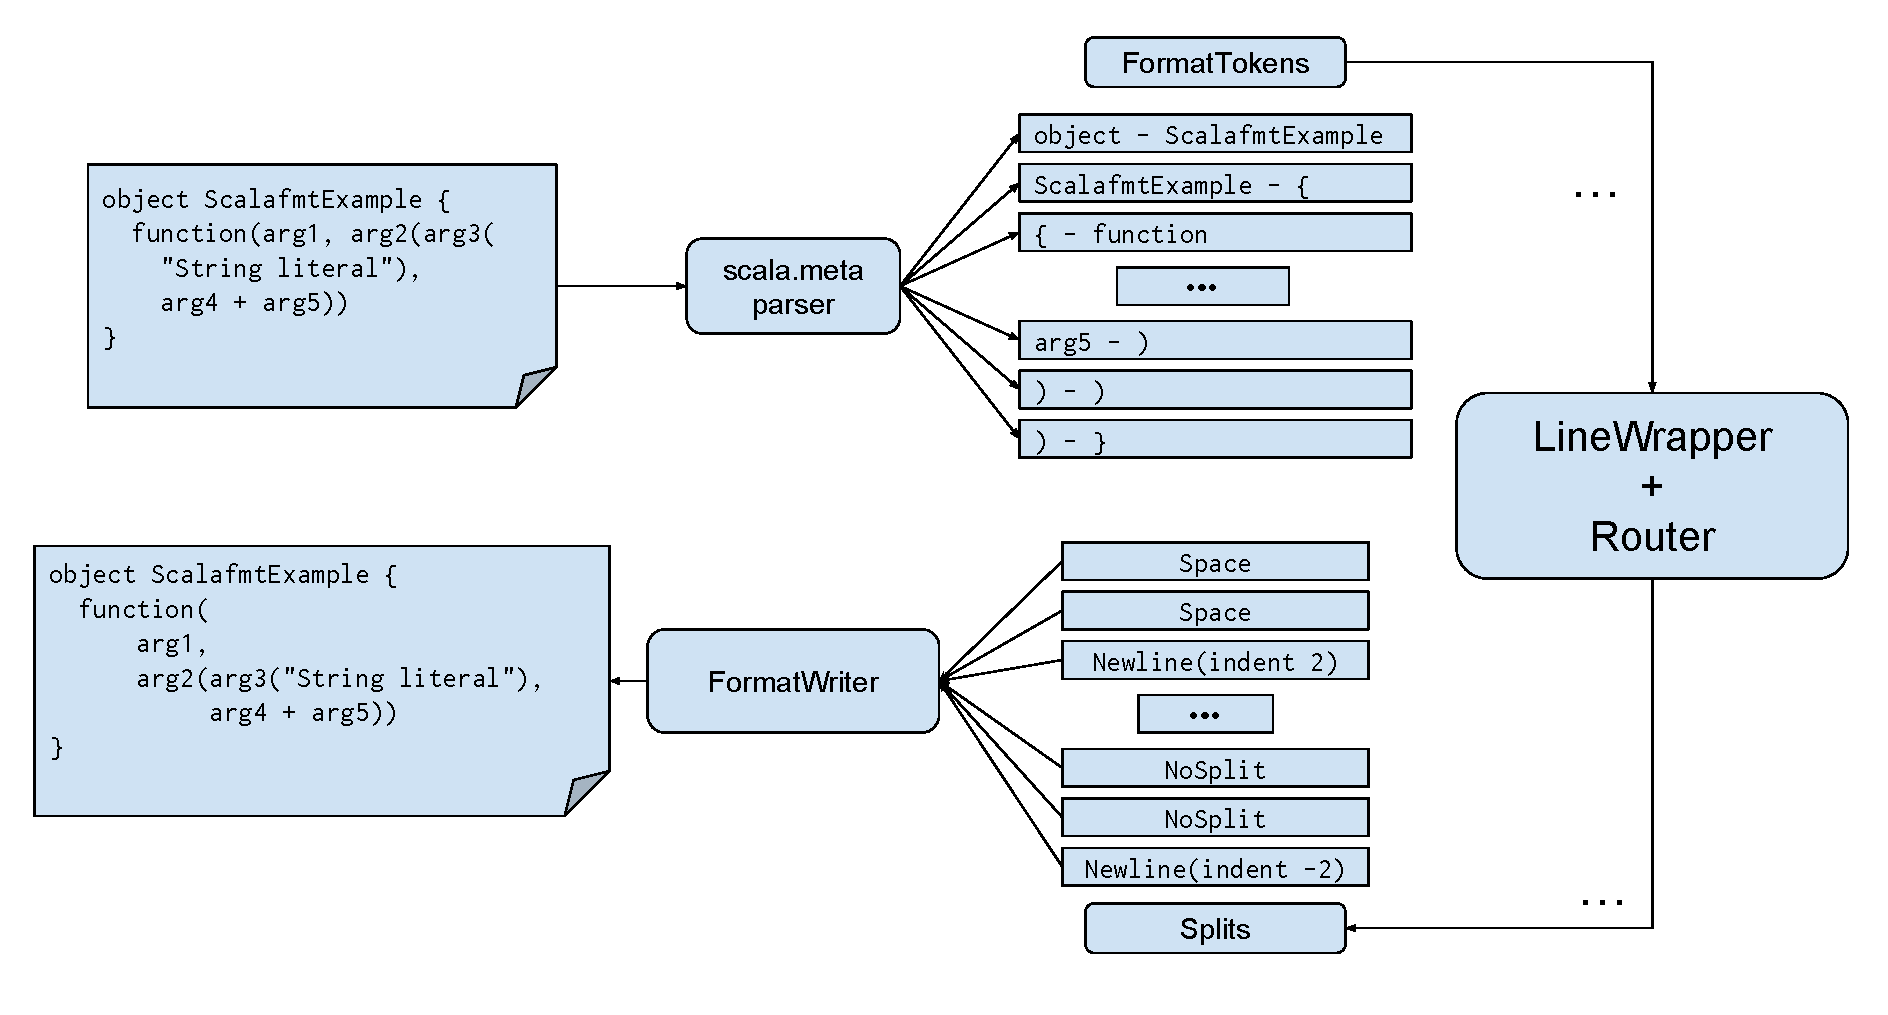
\includegraphics[width=\textwidth]{img/architechture.pdf}
  \caption{Scalafmt architecture}
  \label{fig:architecture}
\end{figure}
First, scalafmt parses a source file using scala.meta.
Next, we feed a sequence of \emph{FormatToken} data types into a \emph{LineWrapper}.
The LineWrapper uses a \emph{Router} to construct a weighted directed graph and run a best-first search to find an optimal formatting layout for the whole file.
Finally, the LineWrapper feeds a sequence of \emph{Split} data types into the \emph{FormatWriter}, which constructs a new reformatted source file.
The following sections explain these data types and abstractions in detail.

\subsection{Data structures}
Scalafmt leverages a few carefully designed data structure to allow an implementation that emphasizes correctness and maintainability.

\subsubsection{FormatToken}
A \emph{FormatToken} is a pair of two non-whitespace tokens.
Listing~\ref{lst:format_token} shows the definition of the FormatToken data type.
\lstinputlisting[label={lst:format_token}, caption=FormatToken definition]{code/format_token.scala}
As shown in the architecture overview in figure~\ref{fig:architecture}, each token except the beginning and end of file tokens appear twice in the sequence of FormatTokens: once as the \texttt{left} member and once as the \texttt{right} member.
In a nutshell, the job of the LineWrapper is to convert each FormatToken into a \emph{Split}

\subsubsection{Decision}\label{sec:decision}
A Decision is a pair of a FormatToken and a sequence of Splits.
Listing~\ref{lst:decision} shows the Definition of decision.
\lstinputlisting[label={lst:decision}, caption=Decision definition]{code/decision.scala}
The \emph{splits} member represents the possible splits that we can take at \emph{formatToken}.

\subsubsection{Policy}\label{sec:policy}
A \emph{Policy} is an enforced formatting layout over a region.
Listing~\ref{lst:policy} shows the definition of Policy.
\begin{minipage}{\linewidth}
  \lstinputlisting[label={lst:policy}, caption=Policy definition]{code/policy.scala}
\end{minipage}
A Policy is a partial function that should be applied to future Decisions up until the \emph{expire} token.
Policies easily compose using the Scala standard library \texttt{orElse} and \texttt{andThen} methods on PartialFunction\footnote{
  Careful eyes will observe that Policy is in fact a monoid with the empty partial function as identity and function composition as associative operator.}.
% The \texttt{isProhibitive} member annotates whether this policy can possibly eliminate Splits from future Decisions.
% This is necessary for an optimization explained in section~\ref{sec:dequeue}.
Policies enable a high-level way to express arbitrary formatting layouts over a region of code.

\subsubsection{Indent}\label{sec:indent}
An \emph{Indent} describes indentation over a region of code.
\lstinputlisting[label={lst:indent}, caption=Indent definition]{code/indent.scala}
Listing~\ref{lst:indent} shows the definition of Indent along with the algebraic data type \emph{Length}.
Length can either be \texttt{Num(n)} where $n$ represents an explicit number of spaces to indent by or \texttt{StateColumn} which is a placeholder the number of spaces required to vertically align by the current column.
Indent is type parameterized by Length so that, at some point, we can replace StateColumn placeholders with Nums to obtain a concrete number.
For example, given a scala.meta tree \texttt{expr}, the definition \texttt{Indent(Num(2), expr.tokens.last, inclusive=true)}
increases the indentation level by 2 spaces up to and including the last token of \texttt{expr}.
The \texttt{inclusive} member is set to false when the indentation should expire before the expire token, for example in a block wrapped by curly braces, since the closing curly brace should not be indented by 2 spaces.
The StateColumn placeholder is required to allow memoization of Splits, which is critical for performance reason as explained in section~\ref{sec:router} on the \emph{Router}.

\subsubsection{Split}
A \emph{Split} represents a (possibly empty) whitespace character to be inserted between two non-whitespace tokens.
Listing~\ref{lst:split} shows the rather intricate definition of the Split data type\footnote{
  For clarity reasons, a few less important members have been removed from the actual Split definition.}.
\begin{minipage}{\linewidth}
  \lstinputlisting[label={lst:split}, caption=Split definition]{code/split.scala}
\end{minipage}
The Split data type went through several generations of design before reaching its current structure.
Each member serves an important role.
The most important member of the Split type is the \emph{modification}.
A modification must be one of \texttt{NoSplit}, \texttt{Space} and \texttt{Newline}.
The \emph{cost} member represents the penalty for choosing this split.
The \emph{optimalToken} member enables an optimization explained in section~\ref{sec:optimal}.
The \emph{indents} member contains the indentation layers that this splits adds.
The \emph{line} member allows a powerful debugging technique explained in section~\ref{sec:router}.
The \emph{policy} and \emph{indents} members are explained in sections~\ref{sec:policy} and~\ref{sec:indent}, respectively.

\subsubsection{State}
A \emph{State} is a partial formatting solution during by the best-first search.
Listing~\ref{lst:state} shows the definition of the State class and companion object.
\begin{minipage}{\linewidth}
  \lstinputlisting[label={lst:state}, caption=State definition]{code/state.scala}
\end{minipage}
Observe the similarity of State and Split.
A State contains various summaries calculated from the \texttt{splits} member.
The summaries are necessary for performance reasons in the best-first search.
Observe that the indents are type parameterized by \texttt{Num}, meaning they only contain concrete indentations and no \texttt{StateColumn} indents.
The \texttt{indentation} member is the sum of all currently active indents and \texttt{column} represents how many characters have been consumed since the last newline.
The State class extends the \texttt{Ordered} trait to allow for efficient polling from a priority queue.
The \texttt{compare} method orders States firstly by their \texttt{totalCost} member, secondly by \texttt{splits.length} -- how many FormatTokens have been formatted -- and finally breaking ties by the \texttt{indentation}.
The method \texttt{nextState} calculates a penalty for characters that overflow the column limit and prepares
The method is implemented as efficiently as possible since the method is on a hot path in the best-first search.

, new summaries to instantiate a new State.
\subsection{LineWrapper}
The LineWrapper is responsible for turning FormatTokens into Splits.
To accomplish this, the LineWrapper employs a \emph{Router} and a best-first search.

\subsubsection{Router}\label{sec:router}
The Router's role is to produce a Decision given a FormatToken.
Figure~\ref{fig:router} shows all possible formatting layout for the small input \texttt{val x = y + z}.
\begin{figure}
  \centering
  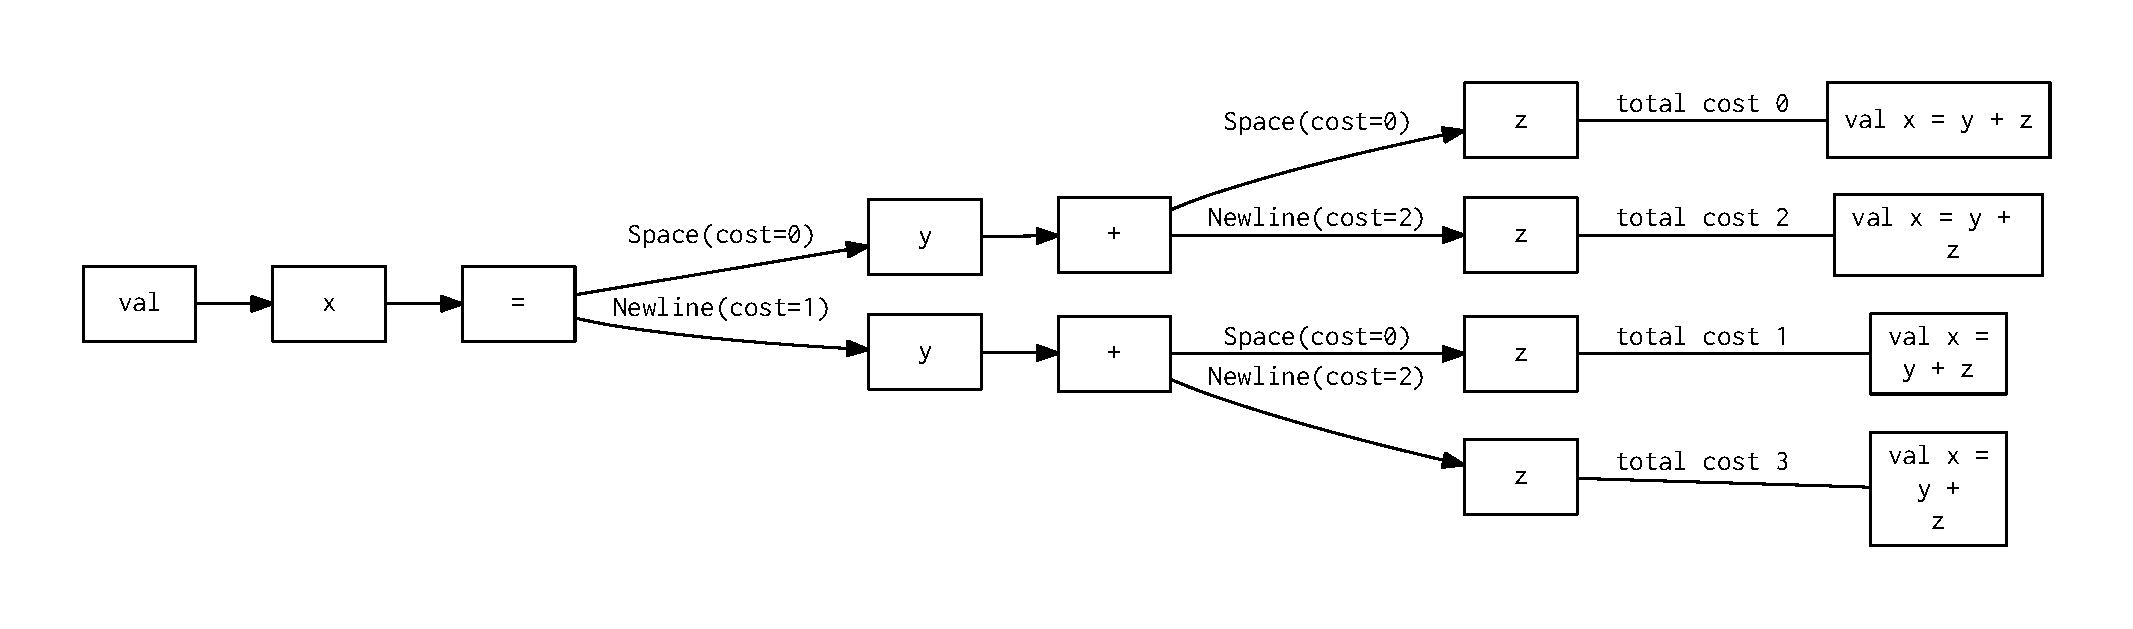
\includegraphics[width=\textwidth]{target/router.pdf}
  \caption{Example graph produced by Router}
  \label{fig:router}
\end{figure}
In this figure, the Router is the planner that chooses which nodes open up multiple branches (\texttt{=} and \texttt{+}) and which nodes have one exit edge only.
This is no easy task since a FormatToken can be any pair of two tokens.
How do we go about implementing a Router?

The Router is implemented as one large pattern match on a FormatToken.
Listing~\ref{lst:match} shows how to pattern match on a FormatToken.
\lstinputlisting[label={lst:match}, caption=Pattern matching on FormatToken]{code/match.scala}
The pattern \texttt{\_: `=`} matches a scala.meta token of type \texttt{`=`}.
The underscore \texttt{\_} ignores the underlying value.
Keyword is a super-class of all scala.meta keyword token types.
Now, a good observer will notice that this pattern match can quickly grow unwieldy long once you account for all of Scala's rich syntax.
How does this solution scale?
Also, once the match grows bigger how can we know from which case each Split origins?
It turns out that Scala's pattern matching and scala.meta's algebraically typed tokens are able to help us.

The Scala compiler can statically detect unreachable code.
If we add a case that is already covered higher up in the pattern match, the Scala compiler issues a warning.
For example, listing~\ref{lst:exhaustive} shows an example where the compiler issues a warning.
\lstinputlisting[label={lst:exhaustive}, caption=Unreachable code]{code/exhaustive.scala}
Here, we accidentally match on a FormatToken with an \texttt{else} keyword on the right which will never match because we have a broader match on a Keyword higher up.
In this small example, the bug may seem obvious but once the Router grows bigger the compiler becomes unmissable.
However, this still leaves us with the second question of finding the origin of each Split.
Scala macros\autocite{burmako2013scala} and implicits\autocite{oliveira2010type} come to the rescue.

The source file line number of where a Split is instantiated is automatically attached on each Split.
Remember in listing~\ref{lst:split} that the Split case class had an implicit member of type \texttt{sourcecode.Line}.
Sourcecode\autocite{lihao91:online} is a tiny Scala library to extract source code metadata from your programs.
The library leverages Scala macros and implicits to unobtrusively surface useful information such as line number of call sites.
Listing~\ref{lst:sourcecode} shows how this works.
\lstinputlisting[label={lst:sourcecode}, caption=Extracting line number from call site]{code/sourcecode.scala}
When a \texttt{sourcecode.Line} not passed explicitly as an argument to Split's constructor, the Scala compiler will trigger its implicit search to fill the missing argument.
The \texttt{sourcecode.Line} companion contains an implicit macro that generates a Line instance from an extracted line number.
Take a moment to appreciate how these two advanced features of the Scala programming language enable a very powerful debugging technique.
The scalafmt router implementation contains 88 cases and spans over 1.000 lines of code.
The ability to trace the origin of each Split has been indispensable in the development of the Router.
% Once the Router can produce Decisions, we can run a best-first search to choose the optimal splits.

\subsubsection{Best-first search}
The Decisions from the Router produce a directed weighted graph, as demonstrated in figure~\ref{fig:router}.
To find the optimal formatting layout, our challenge is to find the cheapest path from the root node to a final node.
The best-first\autocite{pearl_heuristics:_1984} algorithm is an excellent fit for the task.

Best-first search is a graph search algorithm to efficiently traverse a directed weighted graph.
The objective is reach the final token and once we reach there, we terminate the search because we're guaranteed no other solution is better.
Algorithm~\ref{alg:bfsv1} shows a first attempt\footnote{
  Unfortunately, we make heave use of mutation since graph search algorithms typically don't lend themselves well to functional programming principles.
} to adapt a best-first search algorithm to the data structures and terminologies introduced so far.
\begin{algorithm}
  \caption{Scalafmt best-first search, first approach}\label{alg:bfsv1}
  \lstinputlisting[nolol]{code/bfsv1.scala}
\end{algorithm}
In the best case, the search always chooses the cheapest splits and the algorithm runs in linear time.
Observe that the router is responsible for providing well-behaved splits so that we never hit on the error condition after the while loop.
Excellent, does that mean the search is complete?
Absolutely not, this implementation contains several serious performance issues.

Algorithm~\ref{alg:bfsv1} is exponential in the worst case.
For example, listing~\ref{lst:exponential} shows a tiny input that triggers the search to explore over 8 million states.
\lstinputlisting[label={lst:exponential}, caption=Exponential running time]{code/exponential.scala}
Even if we could visit 1 state per microsecond --- reality is closer to 10 states/microsecond ---  the search will take almost 1 second to complete.
This is unacceptable performance to format only 2 lines of code.
Of course, we could special-case long comments, but that would only provide us a temporary solution.
Instead, like with ClangFormat and dartfmt, we must apply several domain specific optimizations.
In the following section, we discuss the optimizations that have shown to work well for scalafmt.

\subsection{Optimizations}
This section explains the most important domain-specific optimizations that were required to get acceptable performance for scalafmt.
We will see that some optimizations are quite ad-hoc and require some creative workarounds.

\subsubsection{dequeueOnNewStatements}\label{sec:dequeue}
Once the search reaches the beginning of a new statement, empty the priority queue.
Observe that the formatting layout for each statement is independent from the formatting layout of the previous statement.
Consider listing~\ref{lst:dequeue}.
\lstinputlisting[label={lst:dequeue}, caption=Two independent statements]{code/dequeue.scala}
Both statements exceed the column limit, which means that the search must back-track to some extent.
However, once the search reaches \texttt{statement2} we have already found an optimal formatting layout for \texttt{statement1}.
When we start backtracking in \texttt{statement2}, there is no need to explore alternative formatting layouts for \texttt{statement1}.
Instead, we can safely empty the search queue once we reach the \texttt{statement2} token.

The \texttt{dequeueOnNewStatements} optimization is implemented by extending algorithm~\ref{alg:bfsv1} with an if statement.
Algorithm~\ref{alg:dequeue} shows a rough sketch of how this is done.
\begin{algorithm}
\caption{dequeueOnNewStatements optimization}\label{alg:dequeue}
  \lstinputlisting[nolol]{code/dequeue-alg.scala}
\end{algorithm}
With an empty queue, we ensure the search backtracks only as far back as is needed.
The \texttt{statementStarts} variable contains all tokens that begin a new statement.
To collect those tokens, we traverse the syntax tree of the input source file and select the first tokens of each statement of a block, each case in a partial function, enumerator in a for comprehension and so forth.
The actual implementation is quite elaborate and is left out of this thesis for clarity reasons.
Unfortunately, our optimization has one small problem.

Algorithm~\ref{alg:dequeue} may dequeue too eagerly inside nested scopes, leading the search to hit the error condition.
Listing~\ref{lst:noopt} shows an example where this happens.
\lstinputlisting[label={lst:noopt}, caption=Overeager dequeueOnNewStatements]{code/noopt.scala}
Remember that each case of a partial function starts a new statement.
The \texttt{dequeueOnNewStatements} optimization will dequeue the queue on the first state that reaches the \texttt{case} token.
In this example, the first state to reach the \texttt{case} token will have a strict Policy that disallows newlines up until the closing parenthesis.
However, we must insert a newline after the comment.
This causes the search to terminate too early and reach the error condition.
By inspecting where this problem occurred, we came up with a simple rule to identify regions where the \texttt{dequeueOnNewStatements} optimization should be disabled.
The simple rule is to never run \texttt{dequeueOnNewStatements} inside a pair of parentheses.
In section~\ref{sec:tooling}, we discuss techniques we used to be confident that this rule indeed works as intended.
In the following section (\ref{sec:recurseOnBlocks}) we explain the \texttt{recurseOnBlocks} optimization, which allows us to reenable \texttt{dequeueOnNewStatements} for selected regions inside parentheses.

\subsubsection{recurseOnBlocks}~\label{sec:recurseOnBlocks}
If the \texttt{dequeueOnNewStatements} optimization is disabled and we start a new block delimited by curly braces, recursively run the best-first search inside the block.
The intuition here is that by recursively running the best-first search, we keep the priority queue small at each layer of recursion.
This allows us to run aggressive optimizations such as \texttt{dequeueOnNewStatements}.

The \texttt{recurseOnBlocks} optimization enables scalafmt to handle idiomatic Scala code where large bodies of higher order functions and blocks are passed around as arguments.
Remember from section~\ref{sec:scala} that  Scala makes it syntactically convenient to in higher order functions as arguments to other functions.
Listing~\ref{lst:recurse} shows an example where this happens and we trigger the \texttt{recurseOnBlocks} optimization.
\lstinputlisting[label={lst:recurse}, caption=recurseOnBlocks example]{code/recurse.scala}
The \texttt{dequeueOnNewStatements} optimization is disabled inside argument list.
The priority queue grows out bounds because the higher order function can have an arbitrary number of statements.

To implement the \texttt{recurseOnBlocks} optimization, we add an extension to algorithm~\ref{alg:bfsv1}.
Algorithm~\ref{alg:recurse} shows a rough sketch of how \texttt{recurseOnBlocks} is implemented.
\begin{algorithm}
\caption{recurseOnBlocks optimization}\label{alg:recurse}
  \lstinputlisting[nolol]{code/recurse-alg.scala}
\end{algorithm}
We change the signature to accept a starting State and token where we stop the search.
Observe that we guard against infinite recursion by not making a recursive call on \texttt{start.formatToken}.
With \texttt{recurseOnBlocks} and \texttt{dequeueOnNewStatements}, we have solved most problems caused by independent statements affecting the formatting layouts of each other.
Next, we leverage recursion again to help the search queue stay small.

\subsubsection{OptimalToken}\label{sec:optimal}
An OptimalToken is a hint from a Split to the best-first search that enables the search to early eliminate competing Splits.
Recall from listing~\ref{lst:split} that a Split has an \texttt{optimalToken} member.
Listing~\ref{lst:optimalToken} shows the definition of OptimalToken.
\lstinputlisting[label={lst:optimalToken}, float, caption=OptimalToken definition]{code/optimalToken.scala}
When the best-first search encounters a Split with a defined OptimalToken,
the best-first search makes an attempt to reach that token with a budget of 0 cost.
If successful, the search can eliminate the competing Splits.
If unsuccessful and the \texttt{killOnFail} member is true, the best-first search eliminates the Split.
Otherwise, the best-first search continues as usual.

By eliminating competing branches, we drastically minimize the search space.
Listing~\ref{lst:optimal} shows an example where the OptimalToken can be applied.
\lstinputlisting[label={lst:optimal}, float, caption=OptimalToken example]{code/optimal.scala}
Scalafmt supports 4 different ways to format call-site function applications.
This means that there will be $4^N$ number of open branches when the search reaches \texttt{UserObject} $N$.
To overcome this issue, we define an OptimalToken at the closing parenthesis.
The best-first search successfully fits the argument list of each \texttt{UserObject} on a single line, and eliminates the 3 other competing branches.
This makes the search run in linear time as opposed to exponential.

To implement the \texttt{OptimalToken} optimization, we add an extension to algorithm~\ref{alg:recurse}.
Algorithm~\ref{alg:optimal} sketches how the extension works.
\begin{algorithm}
  \caption{OptimalToken optimization}\label{alg:optimal}
  \lstinputlisting[nolol]{code/optimalToken-alg.scala}
\end{algorithm}
The \texttt{bestFirstSearch} method has a new \texttt{maxCost} parameter, which is the highest cost that a new splits can have.
Next, if a Split has defined an \texttt{OptimalToken} we make an attempt to format up to that token.
If successful, we update \texttt{optimalFound} variable to eliminate other Splits from being added to the queue.
If unsuccessful and \texttt{killOnFail} is true, we eliminate the Split that defined the OptimalToken.
A straightforward extension to this algorithm would be to add a \texttt{maxCost} member to the \texttt{OptimalToken} definition from listing~\ref{lst:optimalToken}.
However, this has not been necessary for scalafmt.

\subsubsection{pruneSlowStates}
The pruneSlowStates is a optimization that eliminates states that progress slowly.
A state progresses slowly if it visits a token after other equally or less expensive states.
The insight is that if two equally expensive states visit the same token, the first state to visits that token typically produces a better formatting layout.

By eliminating slow states, we obtain a better formatting output in addition to minimizing the search space.
Listing~\ref{lst:slow} shows two equally expensive formatting solutions where one solution is fast and other is slow.
\lstinputlisting[label={lst:slow}, caption=Slow states]{code/slow.scala}
Of course, the line break after \texttt{g +} could be more expensive than the line break after \texttt{c +}.
Instead, the Router is free to assign an identical cost to both line breaks and let \texttt{pruneSlowStates} take care of eliminating the slow state.

The \texttt{pruneSlowStates} is implemented as a extension to algorithm~\ref{alg:optimal}.
Algorithm~\ref{alg:slow} shows a rough sketch of how the extension works.
\begin{algorithm}[H]
  \caption{pruneSlowStates optimization}\label{alg:slow}
  \lstinputlisting[nolol]{code/slow-alg.scala}
\end{algorithm}
Observe that this algorithm is transparent to the Router.
No special annotations are required from Splits.

\subsubsection{escapeInPathologicalCases}
Alas, despite our best efforts to keep the search space small, some inputs can still trigger exponential running times.
The \texttt{escapeInPathologicalCases} optimization is our last resort to handle such pathological inputs.
How do we detect that the search has encountered such a challenging input?

We detect the search space is growing out of bounds by tallying the number of visits per token.
If we visit the same token $N$ times, we can estimate the current branching factor to be around $log_2(N)$.
In scalafmt, we tune $N$ to be 256 so that the best-first search can split into two or more paths for up to 8 tokens.
When a token has been visited more than 256 times, we trigger the \texttt{escapeInPathologicalCases} optimization.
In the following paragraphs section, we present two alternative fallback strategies: \emph{leave unformatted} and \emph{best-effort}.

The simplest and most obvious fallback strategy is to leave the pathologically nested code unformatted.
This can be implemented by backtracing to the first token of the current statement and then reproduce the formatting input up to the last token of said statement.
This method is guaranteed to run linearly to the size of the input.
The responsibility is left to the software developer to a manually format her code, removing all the benefits of code formatting.
However, in some cases the software developer may prefer to get a decent yet suboptimal formatting output.

The best-effort fallback strategy applies heuristics to give a decent but suboptimal formatting output.
When a token is visited for the 256th time, we select two candidate states from the search queue and eliminate all other states.
The first state is the fastest state --- the state that has reached furthest into the token stream --- that is not bound a prohibitive single line policy.
Single line policies are policies that eliminate newline Splits.
The second state is the current state --- the slow state that visited the token for the 256th time.
The intuition is that the fast state has good formatting output so far but for is stuck on a challenging token for some reason.
The slow may paid a hefty penalty early causing it to move slowly but maybe the early penalty will yield a better output in the end.
Algorithm~\ref{alg:best-effort} shows an example of the best-effort strategy can be implemented as an extension to algorithm~\ref{alg:bfsv1}.
\begin{algorithm}
  \caption{best-effort fallback strategy}\label{alg:best-effort}
  \lstinputlisting[nolol]{code/best-effort.scala}
\end{algorithm}
The \texttt{isSafe} method on State returns true if the state contains prohibitive policies, derived from annotated metadata in Splits from the Router.
Observe that this algorithm will reapply the best-effort fallback until the search reaches the final token.
In scalafmt, we bound the number of this can happen with a final fallback to the unformatted strategy.

The unformatted and best-effort fallback strategies offer different trade-offs.
The unformatted strategy works well in a scenario where a software developer is available to manually fix formatting errors.
The best-effort strategy works well on computer generated code where just a modicum of formatting still greatly aid the legibility of the code.
Unfortunately, as we discuss in section~\ref{sec:testing}, we struggled to guarantee idempotency using the best-effort strategy.
This limitation renders the best-effort strategy useless in environments where code formatters are used to enforce a consistent coding style across a codebase.


\subsection{FormatWriter}
Recall from figure~\ref{fig:architecture}, the FormatWriter receives splits from the best-first search and produces a final output presented to the user.
In addition to reifying Splits, the FormatWriter runs three post-processing steps: \emph{docstring formatting}, \emph{vertical alignment} and \emph{stripMargin alignment}.

\subsubsection{Docstring formatting}\label{sec:docstring}
Docstrings are used by software developers to document a specific part of code.
Like in Java, docstrings in Scala start with the \texttt{/**} pragma and end with \texttt{*/}.
However, unlike in Java, the Scala community is split on whether new lines inside docstrings should align by the first or the second asterisk.
The official Scala Style Guide\autocite{Scala80:online} dictates that new lines should align by the second asterisk while the Java tradition is to align by the first asterisk.
The Scala.js\autocite{doeraene_scala.js_2015} and Spark\autocite{xin_spark_2015} style guides follow the Java conventions.
To accommodate all needs, scalafmt allows the user to choose either style.
To enforce that the asterisks are aligned according to the user's preferences,
the FormatWriter rewrites docstring tokens using simple regular expressions.

\subsubsection{stripMargin alignment}
The Scala standard library adds a \texttt{stripMargin} extension method on strings.
The method helps Scala developers write multiline interpolated and regular strings literals.
Listing~\ref{lst:stripMargin} shows an example usage of the \texttt{stripMargin} method.
\lstinputlisting[label={lst:stripMargin}, caption=stripMargin example]{code/stripMargin.scala}
After calling the method, the indentation and \texttt{|} character on line 3 are conveniently stripped away.
However, the hard-fought indentation can easily be lost when the string is moved up or down a scope during refactoring.
Scalafmt can automatically fix the issue.
In the FormatWriter, scalafmt rewrites string literals to automatically align the \texttt{|} characters with the opening triple quotes \texttt{"""}.
This setting is disabled by default since scalafmt has only syntactic information and cannot determine if the \texttt{stripMargin} invocation calls the standard library method or a user-defined method.

\subsubsection{Vertical alignment}

